\documentclass{ctexart}
\textheight 23.5cm \textwidth 15.8cm
\topmargin -1.5cm \oddsidemargin 0.3cm \evensidemargin -0.3cm

\usepackage{verbatim}
\usepackage{fancyhdr}
\usepackage{float}
\usepackage{graphicx}
\usepackage{amssymb}
\usepackage{amsmath}

\pagestyle{fancy}
\CTEXsetup[format = {\Large\bfseries\it}]{section}


\begin{document}

\section*{内容简介}
	\noindent 对函数 
	\begin{equation}
		f(x) = \dfrac{1}{1 + x^2}\qquad x\in[−5,\,5]
	\end{equation}
	构造 Newton 插值多项式 $p_L(x)$,插值结点取为:\\
	
	$1.\ x_i = 5 − \dfrac{10}{N} i \qquad i = 0, 1, \cdots, N$\\
	
	$2.\ x_i = −5\cos\left(\dfrac{2i + 1}{2N + 2}\pi\right) \qquad i = 0, 1, \cdots, N$
	
	\noindent 并计算如下误差
	\begin{equation}
		\max\limits_i\left\{\Big|f(y_i) − p(y_i)\Big|,\quad y_i = \dfrac{i}{10} − 5,\ i = 0, 1, \cdots, 100\right\}
	\end{equation}
	对 $N = 5, 10, 20, 40$ 比较以上两组结点的结果。
	
\section*{工作环境}
	程序所用语言: {\bf python}
	
	软件: {\bf JupyterLab}
	
	使用的包: {\bf numpy,matplotlib}
	
\section*{主要方法}
	Newton 插值多项式,比较法
	
	以下叙述中函数的“收敛”将指函数在无穷范数意义下的收敛。

\section*{输出结果}

\begin{verbatim}
	N = 5
	Max Error of grid (1) : 0.432692307692
	Max Error of grid (2) : 0.555911338812
	N = 10
	Max Error of grid (1) : 1.915643050219
	Max Error of grid (2) : 0.108929039892
	N = 20
	Max Error of grid (1) : 58.278125107739
	Max Error of grid (2) : 0.015325088544
	N = 40
	Max Error of grid (1) : 78689.038205694873
	Max Error of grid (2) : 0.000273859790
\end{verbatim}

\begin{figure}[H]
	\centering
	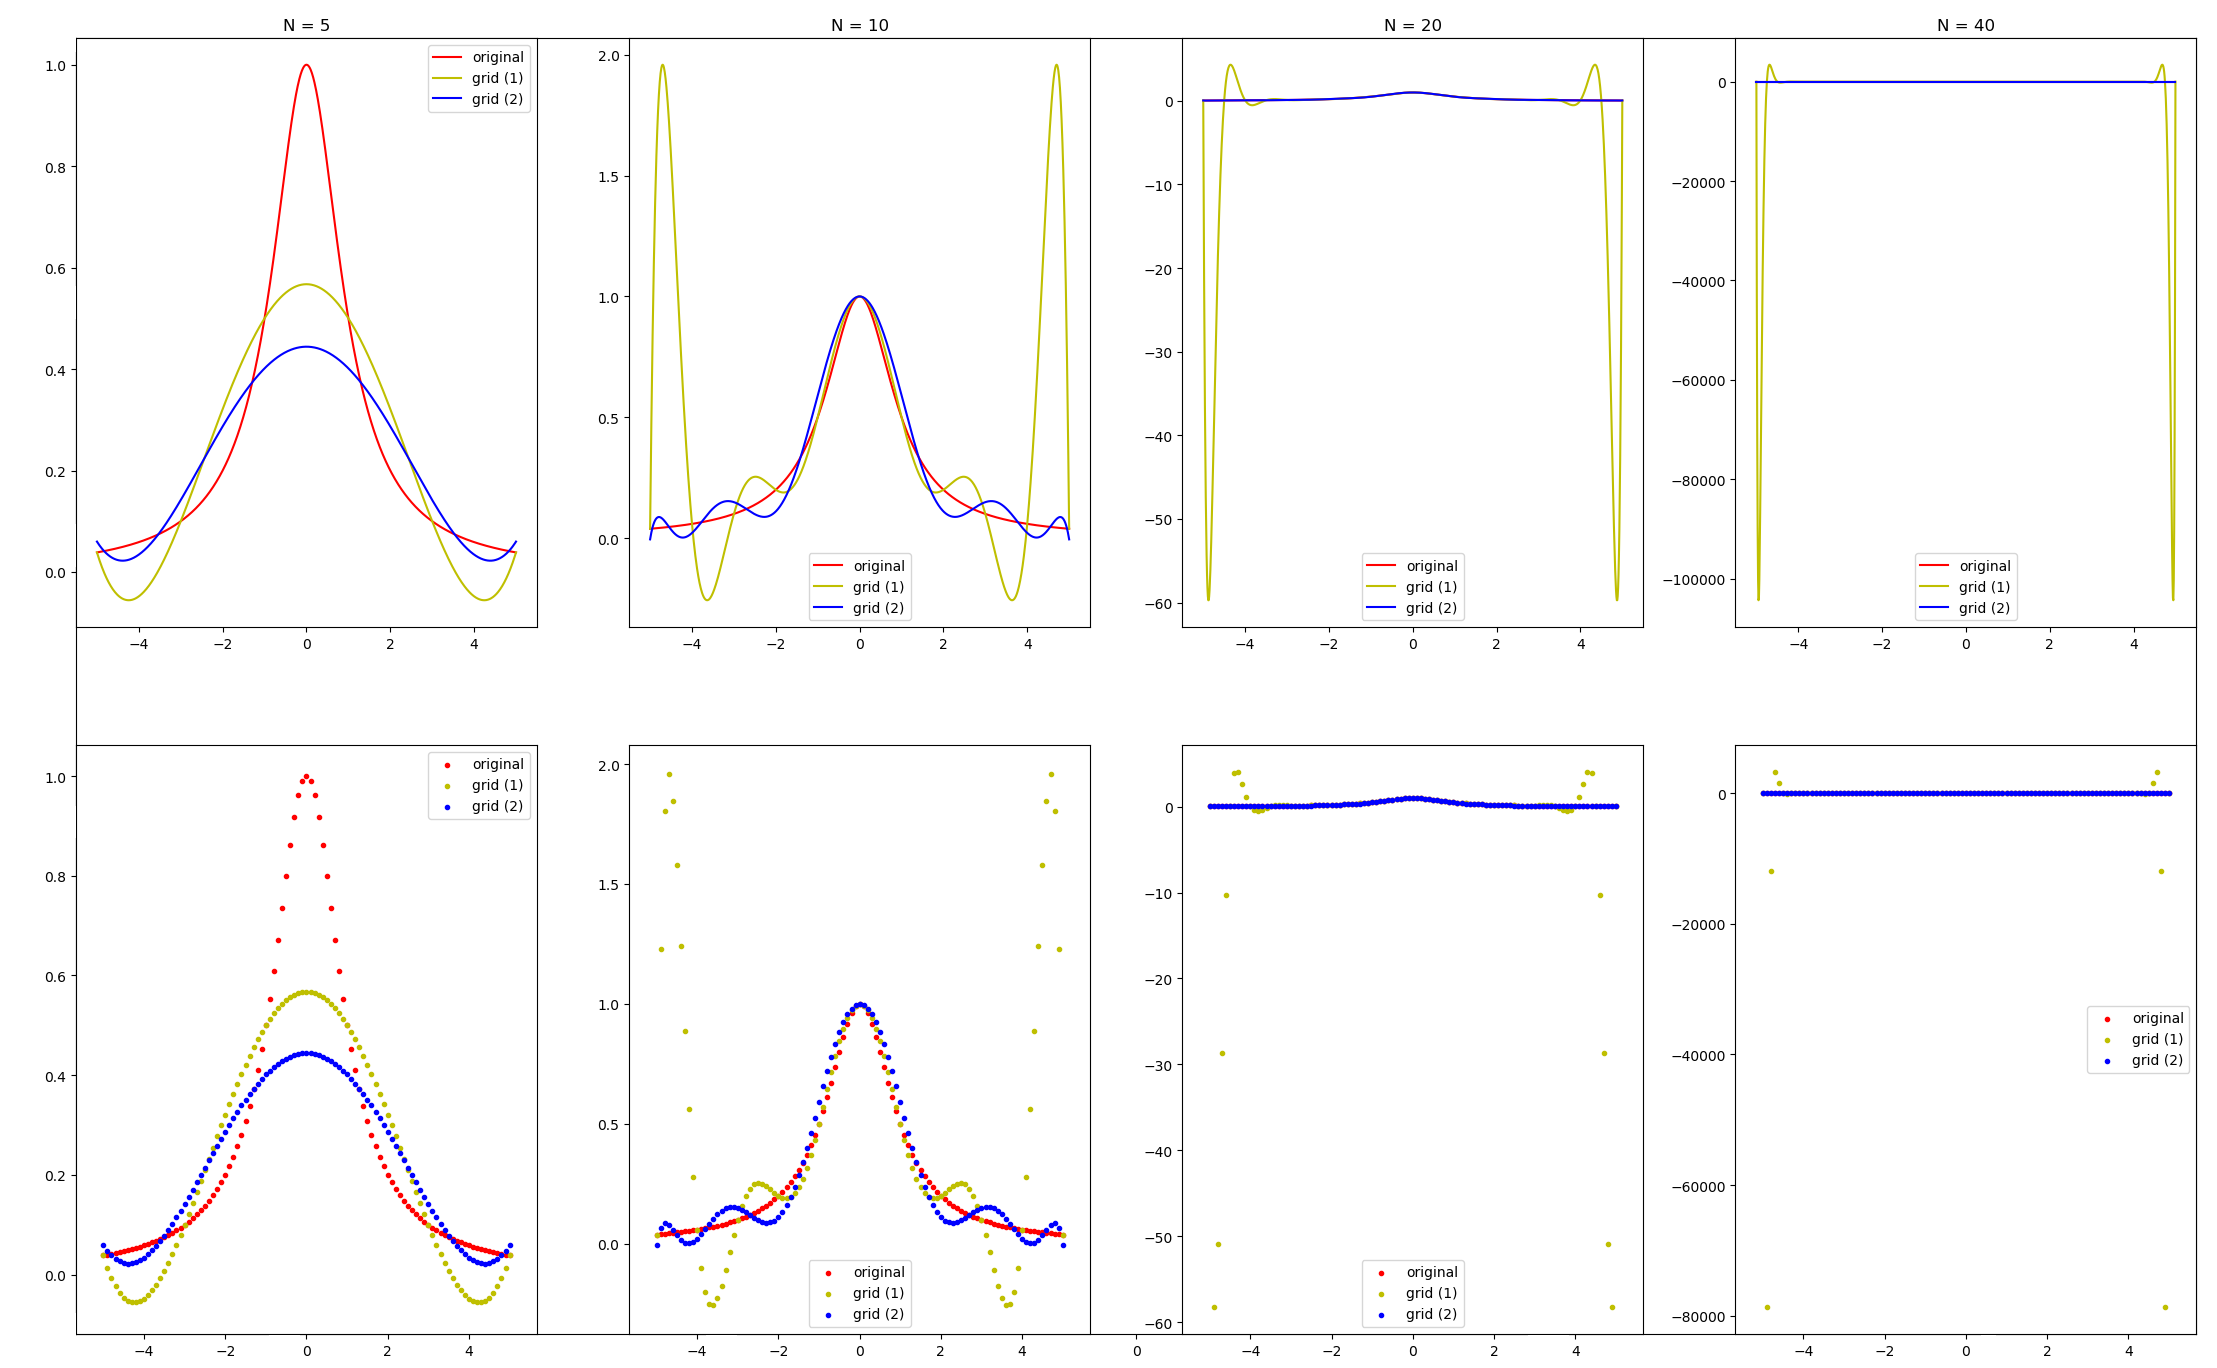
\includegraphics[width = 15cm, height = 8cm]{figure_1.png}
	\caption{整体性质} \label{figure_1.label}
\end{figure}

\begin{figure}[H]
	\centering
	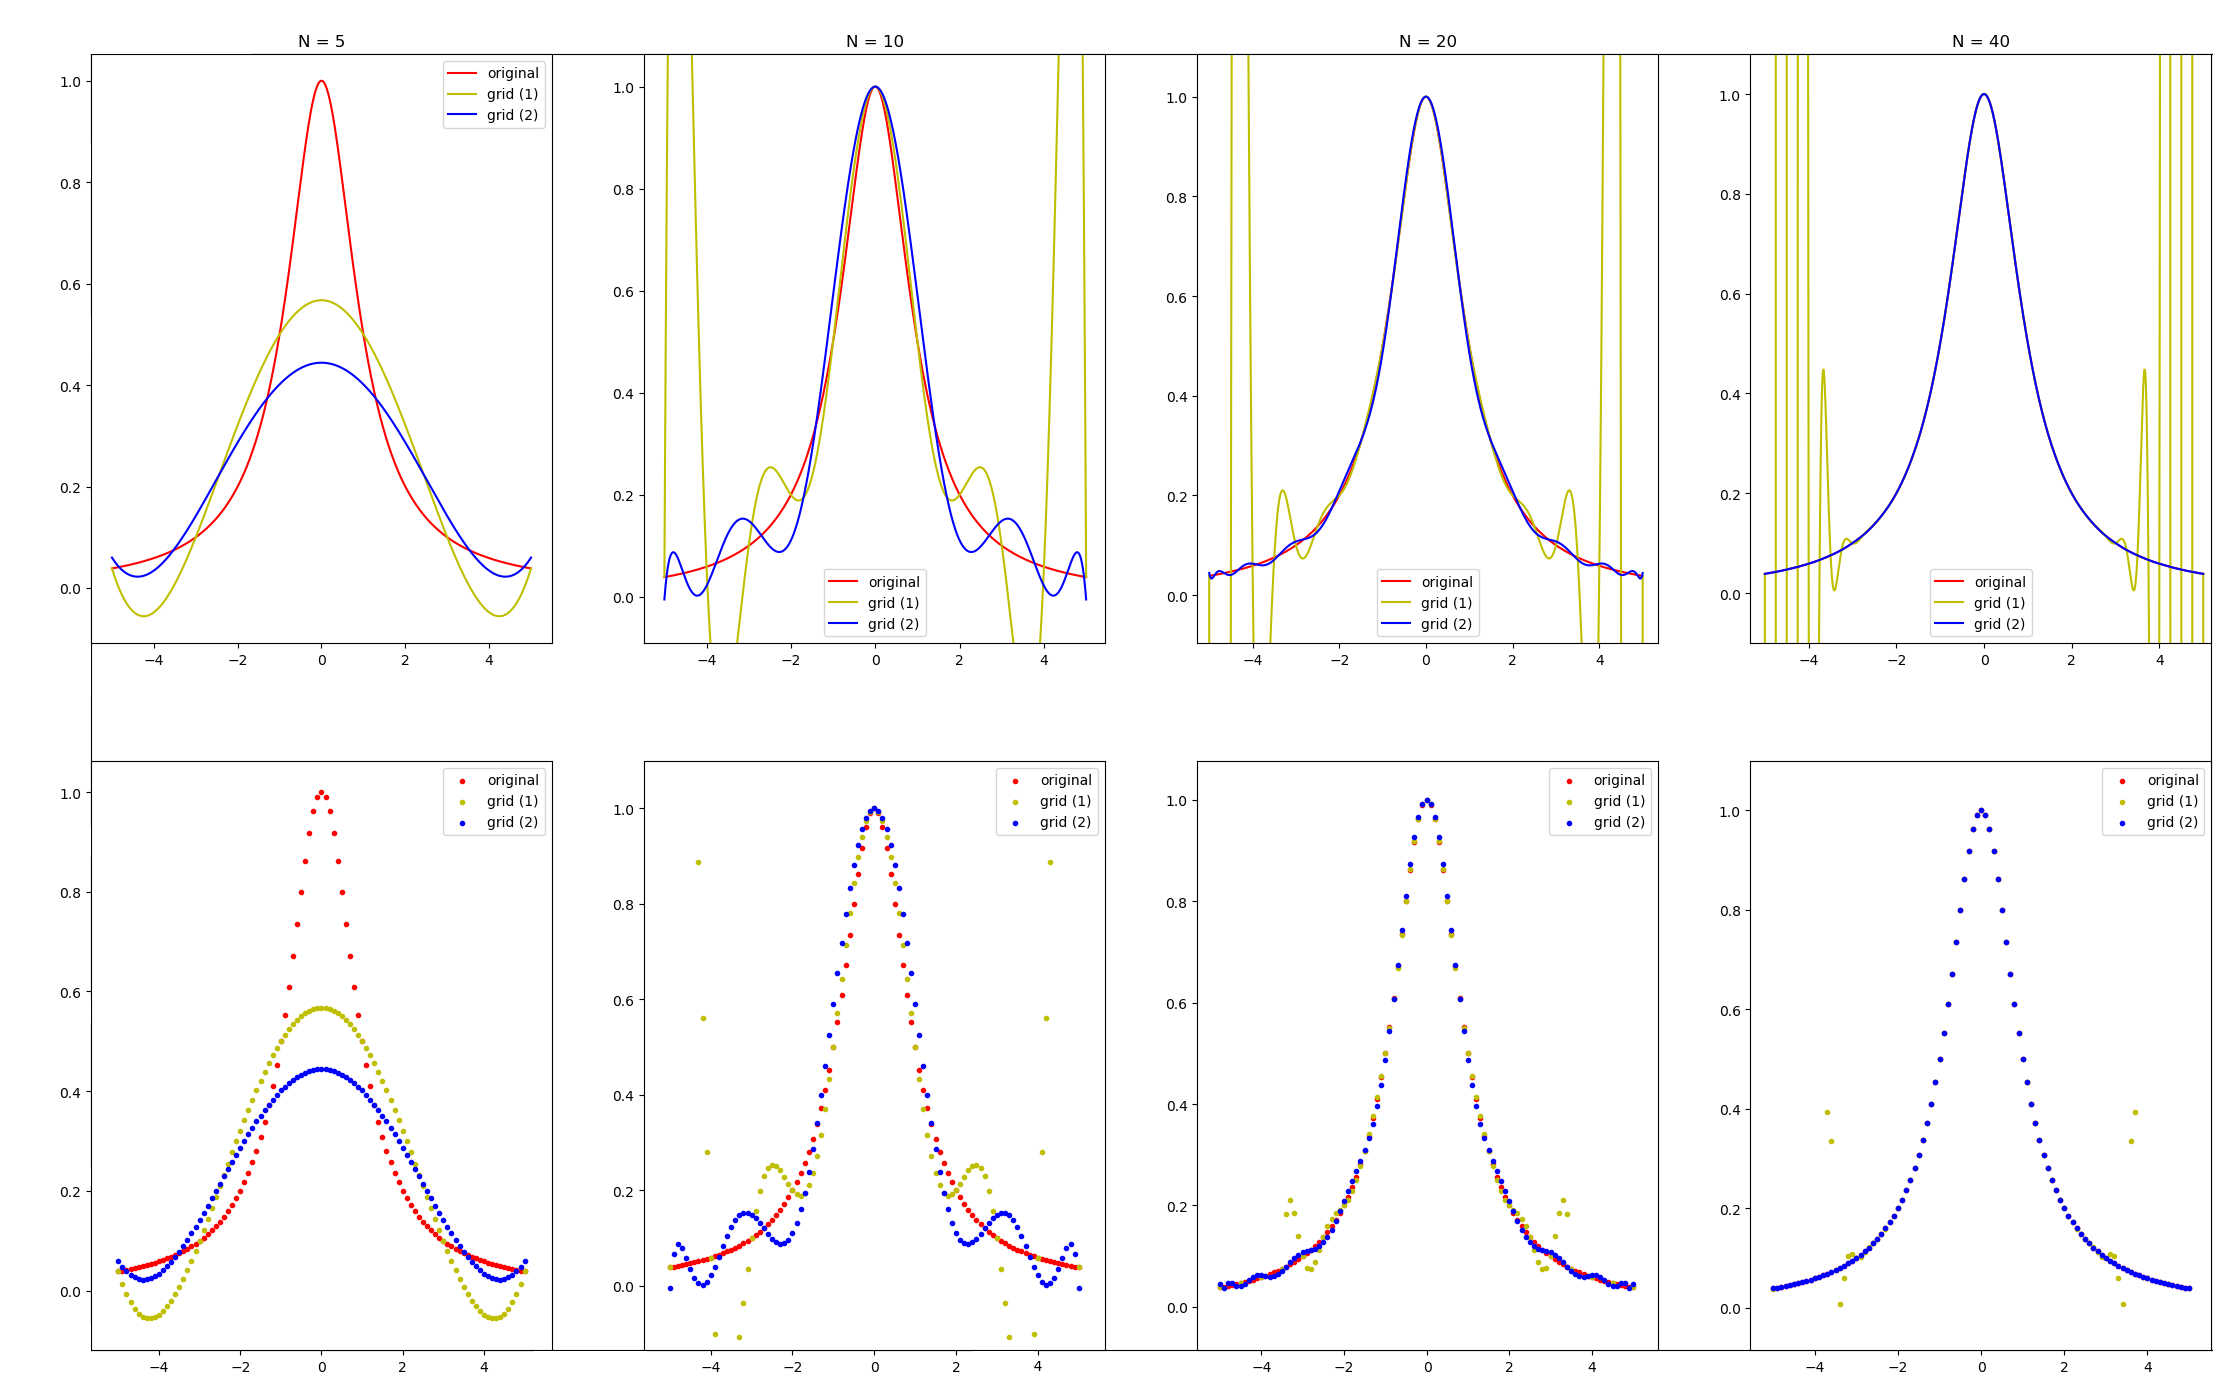
\includegraphics[width = 15cm, height = 8cm]{figure_2.png}
	\caption{局部性质} \label{figure_2.label}
\end{figure}

\begin{table}[htb]
	\centering
	\bigskip
	\begin{small}
		\begin{tabular}{|c|cc|cc|}
			\hline
			n & 等距结点 & order & Chebyshev 结点 & order\\\hline
			5& 4.327E-01 & -- & 5.559E-01 & -- \\
			10& 1.915 & -2.15 & 1.089E-01 & 2.35\\
			20& 5.828E01 & -4.93 & 1.533E-02 & 2.83 \\
			40& 7.869E04 & -10.40 & 2.739E-04 & 5.81\\\hline
		\end{tabular}
	\end{small}
	\caption{\label{table.label} $L_\infty$ 范数意义下的精度检验} 
\end{table}

\section*{现象分析}
	观察到 Newton 插值多项式与作业01的 Lagrange 插值多项式数据点、图像基本一致。这是对于多项式插值唯一性的一个验证。精度检验表明无穷范数意义下误差很有可能非多项式增长速度。\\[2mm]	
	\indent 同作业01,设 $h = \dfrac{10}{N}$,取点 $-5 + \varepsilon$。那么将会得到等距结点下 $||f(x) - p_E(x)||_\infty$ 的一个估计:
	\begin{equation}
		\max{|f(x) - p(x)|} \sim \dfrac{eh^{N+1}}{2(N+1)\sqrt{\pi(N+1)}} \max\limits_{|x| \leqslant 5}{|f^{(N+1)}(\xi_x)|}
	\end{equation}
	
	Chebyshev结点下 $||f(x) - p_C(x)||_\infty$ 的估计:
	\begin{equation}
		\max{|f(x) - p_C(\frac{x}{5})|} \leqslant \dfrac{5^{N+1}}{2^N(N+1)!}\max\limits_{|x| \leqslant 5}|f^{(N+1)}(x)|
	\end{equation}
	因为对于足够大的 $N$,$\dfrac{eh^{N+1}}{2(N+1)\sqrt{\pi(N+1)}} << \dfrac{5^{N+1}}{2^N(N+1)!}$,可知 Chebyshev 结点更有利于收敛。\\
	
	进一步,若比较20位小数下两种插值方法的输出结果:
\begin{verbatim}
	N = 5
	Lagrange
	   Max Error of grid (1) : 0.43269230769230782041
	   Max Error of grid (2) : 0.55591133881239551684
	Newton
	   Max Error of grid (1) : 0.43269230769230770939
	   Max Error of grid (2) : 0.55591133881239551684
	
	N = 10
	Lagrange
	   Max Error of grid (1) : 1.91564305021924785599
	   Max Error of grid (2) : 0.10892903989244862029
	Newton
	   Max Error of grid (1) : 1.91564305021924874417
	   Max Error of grid (2) : 0.10892903989244806517
	
	N = 20
	Lagrange
	   Max Error of grid (1) : 58.27812510773857468394
	   Max Error of grid (2) : 0.01532508854382769181
	Newton
	   Max Error of grid (1) : 58.27812510773861731650
	   Max Error of grid (2) : 0.01532508854382752528
	
	N = 40
	Lagrange
	   Max Error of grid (1) : 78689.03748554707271978259
	   Max Error of grid (2) : 0.00027385978993238469
	Newton
	   Max Error of grid (1) : 78689.03820569487288594246
	   Max Error of grid (2) : 0.00027385978993249571
\end{verbatim}

	可以发现等距结点下,同一插值多项式对于不同的计算方法,计算的函数值有着更大的偏差,有理由猜想这种结点选取方式在计算过程中更容易受到舍入误差的影响。此现象在作业01报告中的{\bf 探索阅读-机器精度因素}部分已说明舍入误差在使用等距结点的 Lagrange 插值多项式计算时有可能被放大。而选取 Chebyshev 结点下插值多项式更易收敛,根据连续性,舍入误差的影响也会相应地降低。
	
\section*{参考资料}
	\noindent [1] David R. Kincaid \& E. Ward Cheney. {\it Numerical Analysis: Mathematics of Scientific of Computing Third Edition}, Brooks/Cole, 2002.

\end{document}